\begin{figure}[h!]
	\centering
	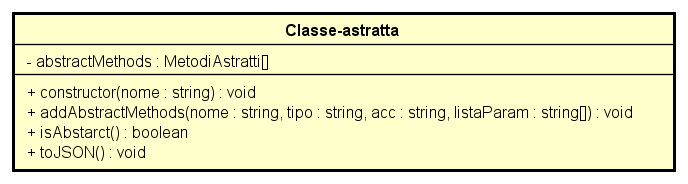
\includegraphics[scale=0.8]{res/sections/SpecificaFrontEnd/Services/Disegnetti/classe-astratta.png}
	\caption{Diagramma della classe Classe-astratta}
\end{figure}

\begin{itemize}
	\item \textbf{Descrizione:}\\
	
	\item \textbf{Utilizzo:}\\
	
	\item \textbf{Attributi:}
		\begin{itemize}
			\item \emph{-abstractMethods: MetodiAstratti[]}\\
			Array contenente i metodi della classe astratta
		\end{itemize}
	\item \textbf{Metodi:}
		\begin{itemize}
			\item \emph{+constructor(nome: string)}\\
    		Costruttore della classe astratta\\
    		\textbf{Parametri:}
    		\begin{itemize}
    			\item \emph{nome: string}\\
    			Nome della classe astratta da creare
    		\end{itemize}
    		\item \emph{+addAbstractMethods(nome: string, tipo: string, acc:string, listaParam: string[])}\\
    		Aggiunge un metodo astratto alla classe\\
    		\textbf{Parametri:}
    		\begin{itemize}
    			\item \emph{nome: string}\\
    			Nome del metodo
    			\item \emph{tipo: string}\\
    			Tipo di ritorno del metodo
    			\item \emph{acc:string}\\
    			Visibilità del metodo
    			\item \emph{listaParam: string[]}\\
    			Lista dei parametri del metodo
    		\end{itemize}
    		\item \emph{+isAbstarct()}\\
    		Ritorna true se l'oggetto è astratto
    		\item \emph{+toJSON()}\\
    		Parsa la classe selezionata e la trasforma in formato JSON
    	\end{itemize}
\end{itemize}